% ACM 投稿模板（acmart, sigconf 双栏版式）
% 文档类由 TeX 发行版提供，首次编译会自动下载所需宏包。
\documentclass[sigconf]{acmart}

% 投稿阶段去掉版权块与页脚的 ACM Reference Format
\settopmatter{printacmref=false}
\renewcommand\footnotetextcopyrightpermission[1]{}
\pagestyle{plain}

\usepackage{booktabs}
\usepackage{multirow}
% acmart 已经加载了 amssymb，再手动加载会与 \Bbbk 冲突，只补 amsmath
\usepackage{amsmath}
\usepackage{graphicx}

\begin{document}

\title{A Compact ACM Format Example with Figures and Tables}

\author{First Author}
\affiliation{%
  \institution{Some University}
  \city{Beijing}
  \country{China}}
\email{first@example.edu}

\author{Second Author}
\affiliation{%
  \institution{Another Institute}
  \city{Shanghai}
  \country{China}}
\email{second@example.edu}

\begin{abstract}
This sample document demonstrates the ACM \texttt{acmart} class with a
two-column layout, an included bitmap figure, a professional
\texttt{booktabs} table, a merged-cell table and a numbered equation.
Replace the content with your own manuscript.
\end{abstract}

\keywords{template, acmart, figures, tables}

\maketitle

\section{Introduction}
ACM papers use the two-column \texttt{sigconf} layout. Keep figures at
\verb|\columnwidth| so they fit inside a single column, and use
\verb|\textwidth| only for wide floats that span both columns.
Related work builds on the Transformer~\cite{vaswani2017attention} and
residual networks~\cite{he2016deep}.

\section{Figures}
Figure~\ref{fig:curve} is inserted with \verb|\includegraphics| at
\verb|\columnwidth|. PNG, JPG and PDF are all supported by the
underlying graphics driver.

\begin{figure}[t]
  \centering
  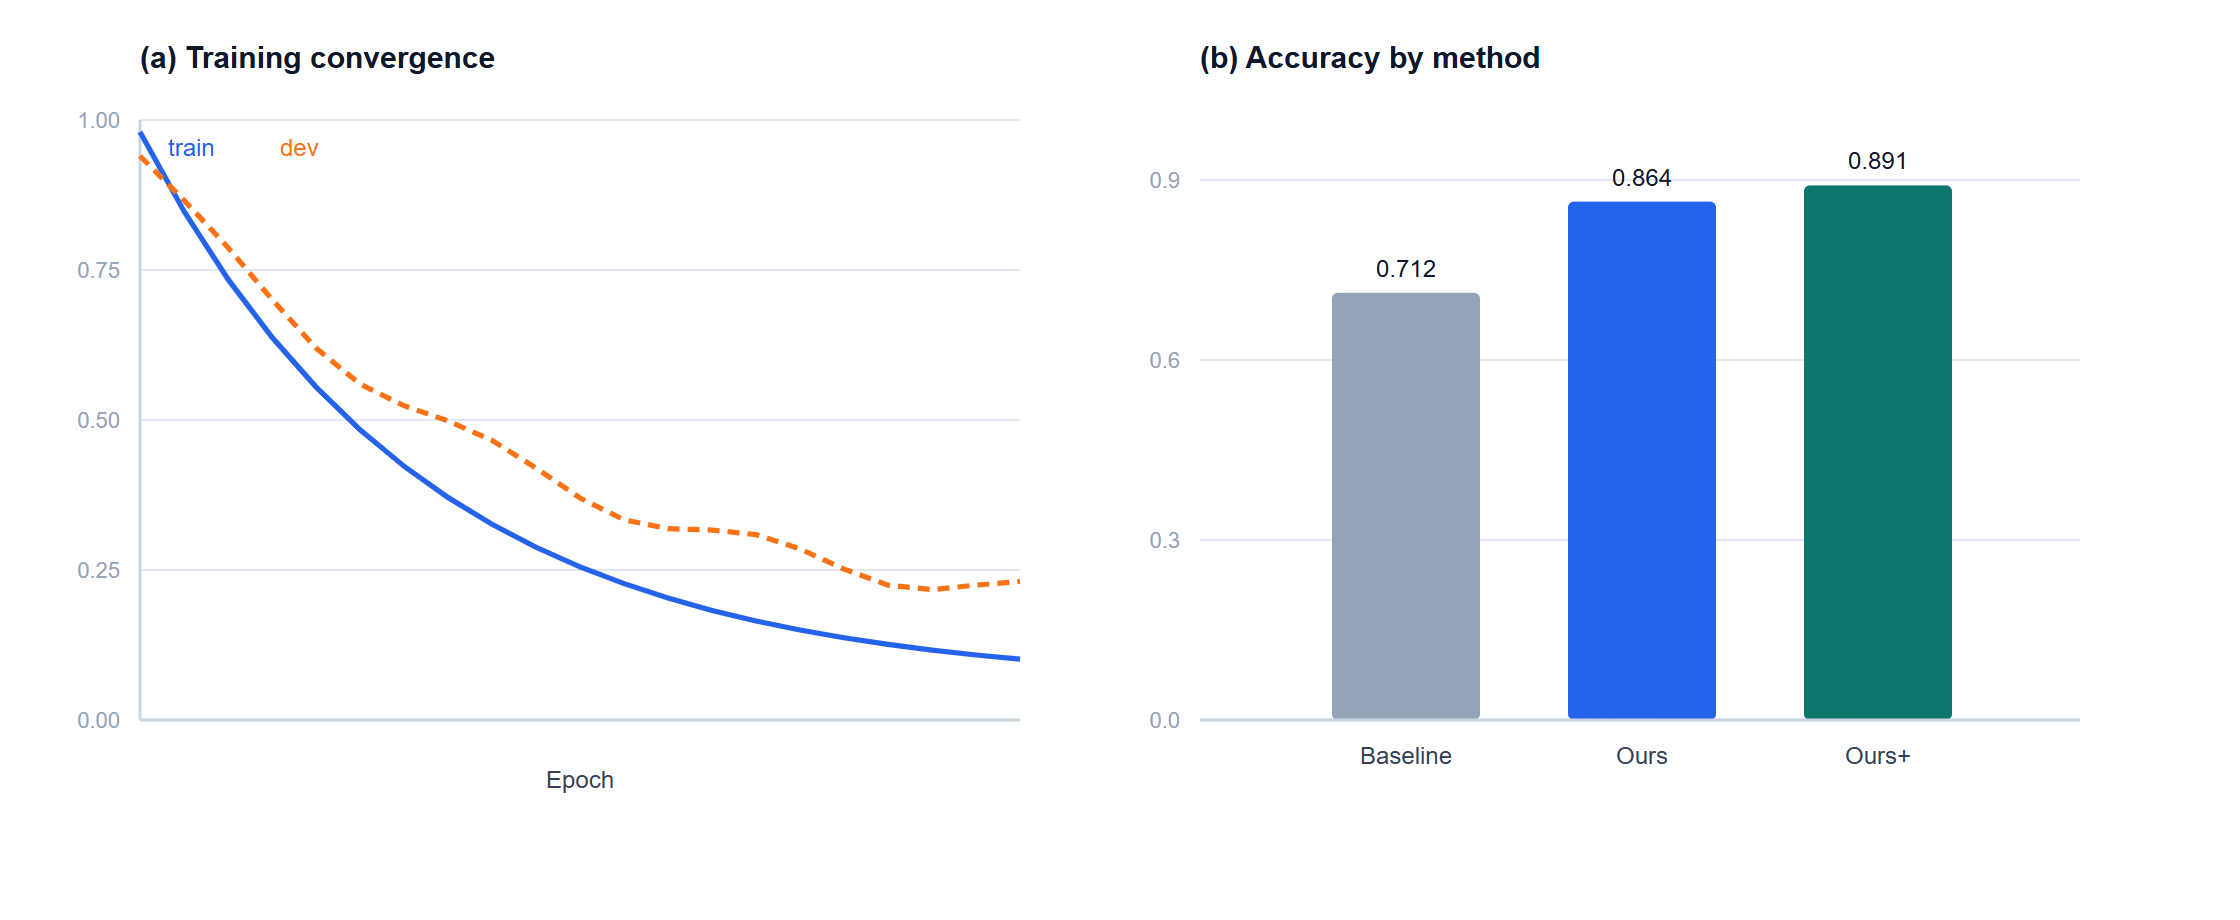
\includegraphics[width=\columnwidth]{figure.png}
  \caption{Training convergence and accuracy comparison. A bitmap
    figure included at column width.}
  \Description{Two panels: a convergence curve and a bar chart.}
  \label{fig:curve}
\end{figure}

\section{Tables}
Table~\ref{tab:main} uses \texttt{booktabs} rules, and
Table~\ref{tab:merged} shows merged cells with \texttt{multirow} and
\texttt{multicolumn}.

\begin{table}[t]
  \caption{Accuracy of different methods.}
  \label{tab:main}
  \centering
  \begin{tabular}{lcc}
    \toprule
    Method & Dev & Test \\
    \midrule
    Baseline & 0.712 & 0.705 \\
    Ours     & 0.864 & 0.871 \\
    Ours+    & \textbf{0.891} & \textbf{0.883} \\
    \bottomrule
  \end{tabular}
\end{table}

\begin{table}[t]
  \caption{Backbone comparison with merged header cells.}
  \label{tab:merged}
  \centering
  \begin{tabular}{llc}
    \toprule
    \multirow{2}{*}{Model} & \multirow{2}{*}{Backbone} & Accuracy \\
    \cmidrule(l){3-3}
     & & (test) \\
    \midrule
    Ours  & ViT-B & 0.871 \\
    Ours+ & ViT-L & 0.883 \\
    \bottomrule
  \end{tabular}
\end{table}

\section{Equations}
The Gaussian density in Equation~\eqref{eq:gauss} is a typical inline
and display math example.

\begin{equation}
  f(x)=\frac{1}{\sqrt{2\pi}\,\sigma}
  \exp\!\left(-\frac{(x-\mu)^2}{2\sigma^2}\right)
  \label{eq:gauss}
\end{equation}

\section{Conclusion}
Compile with the default engine; \texttt{acmart} and
\texttt{ACM-Reference-Format} are resolved automatically.

\bibliographystyle{ACM-Reference-Format}
\bibliography{refs}

\end{document}
